%%%%%%%%%%%%%%%%%%%%%%%%%%%%%%%%%%%%%%%%%%%%%%%%%%%%%%%%%%%%%%%%%%%%%
\subsection{Increasing Pipeline Parallelism by Repartitioning Memories (8 marks)}\label{sec:1c}
%%%%%%%%%%%%%%%%%%%%%%%%%%%%%%%%%%%%%%%%%%%%%%%%%%%%%%%%%%%%%%%%%%%%%

The work in this section is based on L2 pipelining with auto pipelining enabled using T2P memory.
The loop details for this baseline is in \autoref{tab:float-loop-1c0-baseline-ap-l2}.

%%%%%%%%%%%%%%%%%%%%%%%%%%%%%%%%%%%%%%%%%%%%%%%%%%%%%%%%%%%%%%%%%%%%%
\subsubsection{Understanding the \texttt{dim} parameter}\label{sec:1cDim}

Instead of diving into the factor, which is of interest in this project,
we try to choose an appropriate \texttt{dim}.
The \texttt{dim} option is used to specify which dimension is partitioned.
\autoref{fig:float-partition-dim} is a figure coming from \textit{Vitis HLS User Guide (ug1399)}, which clearly shows the idea of \texttt{dim}.
In our application, the loop body of L2 is pipelined, which reads 256 elements from \texttt{in\_buf} and 256 elements from \texttt{weight\_buf}.
In order to improve parallelism, it is obvious that we should distribute the one vector of 256 elements to several blocks of memory.
That is, we need to set \texttt{dim} to 2.

\begin{figure}[ht!]
    \centering
    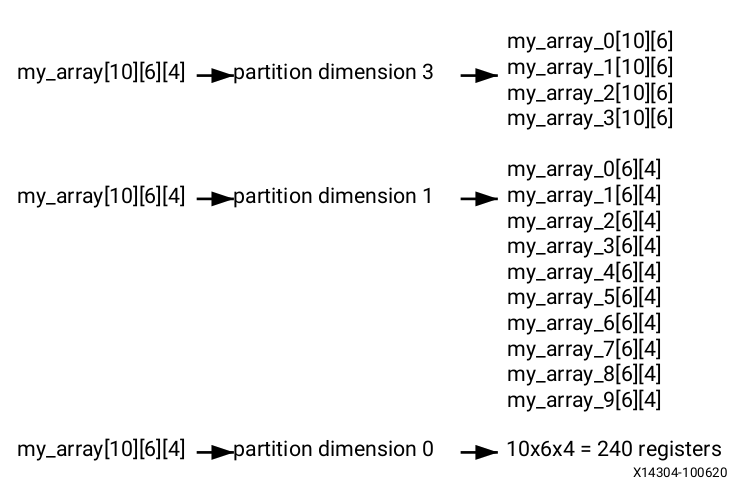
\includegraphics[scale=0.5]{images/float-partition-dim.png}
    \caption{Partitioning Array Dimensions}
    \label{fig:float-partition-dim}
\end{figure}

\begin{figure}[ht!]
    % \centering
    \begin{subfigure}[b]{\textwidth}
        \inputminted[firstline=3]{diff}{program/1c1-partition-ap-d1-f2.diff}
        \caption{Setting array partition with \texttt{dim}=1}
        \label{fig:1c1-partition-ap-d1-f2.diff}
    \end{subfigure}
    \begin{subfigure}[b]{\textwidth}
        \inputminted[firstline=3]{diff}{program/1c1-partition-ap-d2-f2.diff}
        \caption{Setting array partition with \texttt{dim}=2}
        \label{fig:1c1-partition-ap-d2-f2.diff}
    \end{subfigure}
    \caption{Comparing different setting of \texttt{dim}}\label{fig:1c1-partition-d12}
\end{figure}

I have also experimented on this, where the code is modified as \autoref{fig:1c1-partition-d12}.
The HLS summary (\autoref{tab:float-summary}) shows setting \texttt{dim} to 1 introduces more resource usage but the latency is worse.
On the contrary, setting \texttt{dim} to 2 leads to introducing more floating-point adders and multipliers and achieves a lower latency.
The result also supports our conclusion above.

%%%%%%%%%%%%%%%%%%%%%%%%%%%%%%%%%%%%%%%%%%%%%%%%%%%%%%%%%%%%%%%%%%%%%
\subsubsection{Trying different \texttt{factor}s}\label{sec:1cFac}

As shown in \autoref{tab:float-summary}, adding the \texttt{factor} to 32 makes the utilization of DSP and LUT exceeds the resource budget.

When \texttt{factor}=8, the latency is reduced to 4911, which means 46.4x improvement, where 16 floating-point adders and 16 floating-point multipliers are used.
When \texttt{factor}=16, the latency is reduced to 4279, which means 53.3x improvement, where 32 floating-point adders and 32 floating-point multipliers are used.
That is exactly 16 times of that when array partition is not used.
From \autoref{tab:float-loop-1c2-partition-ap-d2-f8} and \autoref{tab:float-loop-1c2-partition-ap-d2-f16}, it can be seen that the initiation interval is 16 cyles when \texttt{factor}=8 and 8 cycles when \texttt{factor}=16.

\begin{table}[ht!]
    \caption{Loop details for partition with \texttt{dim}=2 \texttt{factor}=8}
    \label{tab:float-loop-1c2-partition-ap-d2-f8}
    \centering
    \begin{tabularx}{\textwidth}{ p{4cm} *{7}{C}}
    \toprule
    \multicolumn{1}{c}{\multirow{2}{*}{Loop Name}} &
    \multicolumn{2}{c}{Latency (cycles)}           &
    \multicolumn{1}{c}{\multirow{2}{*}{\makecell*{Iteration \\
    Latency}}}                                     &
    \multicolumn{2}{c}{Initiation Interval}        &
    \multicolumn{1}{c}{\multirow{2}{*}{\makecell*{Trip      \\
    Count}}}                                       &
    \multicolumn{1}{c}{\multirow{2}{*}{Pipelined}}          \\

    \cmidrule(lr){2-3}
    \cmidrule(lr){5-6}

                                                   &
    \multicolumn{1}{c}{min}                        &
    \multicolumn{1}{c}{max}                        &
                                                   &
    \multicolumn{1}{c}{achieved}                   &
    \multicolumn{1}{c}{target}                     &        \\
    \midrule
    \texttt{- LOAD\_OFF\_1} & 5 & 5 & 1 & 1 & 1 & 5 & yes \\
\texttt{- LOAD\_W\_1\_LOAD\_W\_2} & 1280 & 1280 & 1 & 1 & 1 & 1280 & yes \\
\texttt{- LOAD\_I\_1\_LOAD\_I\_2} & 1024 & 1024 & 1 & 1 & 1 & 1024 & yes \\
\texttt{- L1\_L2} & 2550 & 2550 & 1287 & 16 & 1 & 80 & yes \\
\texttt{- STORE\_O\_1\_STORE\_O\_2} & 42 & 42 & 4 & 1 & 1 & 40 & yes \\
    \bottomrule
\end{tabularx}

\end{table}

\begin{table}[ht!]
    \caption{Loop details for partition with \texttt{dim}=2 \texttt{factor}=16}
    \label{tab:float-loop-1c2-partition-ap-d2-f16}
    \centering
    \begin{tabularx}{\textwidth}{ p{4cm} *{7}{C}}
    \toprule
    \multicolumn{1}{c}{\multirow{2}{*}{Loop Name}} &
    \multicolumn{2}{c}{Latency (cycles)}           &
    \multicolumn{1}{c}{\multirow{2}{*}{\makecell*{Iteration \\
    Latency}}}                                     &
    \multicolumn{2}{c}{Initiation Interval}        &
    \multicolumn{1}{c}{\multirow{2}{*}{\makecell*{Trip      \\
    Count}}}                                       &
    \multicolumn{1}{c}{\multirow{2}{*}{Pipelined}}          \\

    \cmidrule(lr){2-3}
    \cmidrule(lr){5-6}

                                                   &
    \multicolumn{1}{c}{min}                        &
    \multicolumn{1}{c}{max}                        &
                                                   &
    \multicolumn{1}{c}{achieved}                   &
    \multicolumn{1}{c}{target}                     &        \\
    \midrule
    \texttt{- LOAD\_OFF\_1} & 5 & 5 & 1 & 1 & 1 & 5 & yes \\
\texttt{- LOAD\_W\_1\_LOAD\_W\_2} & 1280 & 1280 & 1 & 1 & 1 & 1280 & yes \\
\texttt{- LOAD\_I\_1\_LOAD\_I\_2} & 1024 & 1024 & 1 & 1 & 1 & 1024 & yes \\
\texttt{- L1\_L2} & 1918 & 1918 & 1287 & 8 & 1 & 80 & yes \\
\texttt{- STORE\_O\_1\_STORE\_O\_2} & 42 & 42 & 4 & 1 & 1 & 40 & yes \\
    \bottomrule
\end{tabularx}

\end{table}
